\documentclass[conference]{IEEEtran}
% \IEEEoverridecommandlockouts
% The preceding line is only needed to identify funding in the first footnote. If that is unneeded, please comment it out.
\usepackage{cite}
\usepackage[portuguese]{babel}
\usepackage{amsmath,amssymb,amsfonts}
\usepackage{algorithmic}
\usepackage{graphicx}
\usepackage{textcomp}
\usepackage{xcolor}
\usepackage{url}
\def\BibTeX{{\rm B\kern-.05em{\sc i\kern-.025em b}\kern-.08em
    T\kern-.1667em\lower.7ex\hbox{E}\kern-.125emX}}

\title{Sistemas de Informação de Transporte de Mercadorias}
\author{
\IEEEauthorblockN{Pedro Henrique L.B.T Bomfim, Robson França, Igor Nascimento}
\IEEEauthorblockA{\textit{Universidade de São Paulo}}
}
\date{April 2025}

\begin{document}

\maketitle

\begin{abstract}
Este artigo tem como objetivo introduzir os conceitos de sistemas de informação aplicados ao transporte de mercadorias, com base, principalmente, na obra de K. C. Laudon e J. P. Laudon\cite{laudon2015}, oferecendo uma visão abrangente e com foco especial nos Sistemas de Gerenciamento de Transporte (\textit{TMS — Transportation Management Systems}). Serão abordadas suas funcionalidades, componentes, classificação, integração com tecnologias emergentes e a aplicação das Forças de Porter para entender sua importância estratégica. Também serão discutidos exemplos práticos de TMS e WMS (\textit{Warehouse Management System})

\end{abstract}

\section{Introdução}
A intensa globalização e o crescimento do comércio eletrônico colocaram os sistemas de informação (SI) em um papel central no setor de transporte de mercadorias. Contribuindo para a eficiência, segurança e cumprimento de prazos, empresas como os Correios, FedEx, DHL e UPS utilizam esses sistemas para gerenciar o envio de milhões de encomendas diariamente. Entre esses sistemas, destacam-se o TMS e o WMS, sendo o primeiro uma ferramenta essencial para o planejamento, execução e otimização das operações de transporte, e o segundo, um recurso fundamental para a gestão e visibilidade das cadeias de suprimentos.

\section{Caracterização}
O principal objetivo de um Sistema de Informação é coletar, processar, armazenar e distribuir informações para apoiar a tomada de decisões, a coordenação, o controle e a análise de problemas dentro de uma organização. Este SI apresenta uma vasta gama de aplicações, especializações e benefícios.
\subsection{Como TMS}
Ao ser aplicado como TMS, atua como plataforma logística, executando e otimizando a movimentação física de mercadorias, seja na entrada ou saída, geralmente usado como um componente do sistema de gerenciamento de cadeia de suprimentos (SCM) maior. Desempenhando papel central nas cadeias de suprimentos, leva a um planejamento e execução de transporte mais eficientes.

O Sistema de Gerenciamento de Transporte pode ser melhor compreendido ao dividi-lo em partes: software, hardware, pessoas e procedimentos. Existem múltiplos fornecedores de software para este SI, como o \textit{Oracle Transportation Management} (OTM) e o \textit{SAP Transportation Management}, ambos permitem a centralização integrada de recursos logísticos, permitindo uma maior eficiência e redução dos custos. Na questão de hardware, é necessário uma infraestrutura tecnológica, como servidores, computadores, dispositivos móveis e sensores IoT para rastreamento de cargas. Os usuários deste sistema costumam ser os operadores logísticos, gerentes e analistas de transporte, interagindo com o SI para executar tarefas, interpretar dados e tomar decisões.

Uma funcionalidade comum ao TMS é quando este recebe um pedido de entrega, atuando do começo ao fim, o sistema seguiria este procedimento:
\begin{enumerate}
    \item Receber pedido de transporte
    \item Inserir dados no TMS
    \item Gerar rota e selecionar transportadora
    \item Emitir documentos fiscais
    \item Monitorar transporte via IoT
    \item Registrar entrega e gerar relatório de desempenho
\end{enumerate}\cite{oracleTMS}\cite{sapTMS}
\subsection{Como WMS}
Ao ser empregado como WMS, atua oferecendo visibilidade de todo o estoque de uma empresa e gerencia as operações de atendimento da cadeia de suprimentos, e são projetados para dar suporte às necessidades de toda uma cadeia de suprimentos global. Também podem ser estendidos para alinhar o gerenciamento de estoque e serviços de atendimento com métodos de compra modernos, oferecendo visibilidade em tempo real de todo o estoque. Desempenha ajuda ao gerenciamento e controle de operações diárias de depósito de uma empresa.

Também é possível dividir seus principais componentes. Soluções de software como o \textit{SAP Extended Warehouse Management} (SAP EWM) e o \textit{Oracle Warehouse Management Cloud} (WMS Cloud), permitindo funcionalidades como a rastreabilidade de produtos por lote, validade ou localização, usado por operadores de armazém, supervisores logísticos e analistas de logística. O hardware necessário para operar este software são leitores de código de barras (Coletores de dados em geral), servidores ou cloud servers para hospedar o WMS e terminais de consulta. Um processo padrão deste sistema é descrito a seguir:
\begin{enumerate}
    \item Pré-cadastro do pedido no sistema (compra ou transferência).
    \item Chegada da mercadoria no armazém.
    \item Leitura do código de barras dos produtos com o coletor.
    \item Conferência dos itens recebidos (quantidade, lote, validade).
    \item O WMS sugere uma localização com base em regras de armazenagem (ex: tipo de produto, giro, peso).
    \item O operador leva o produto até a localização sugerida.
    \item Confirmação da armazenagem via coletor (scan do endereço de destino).
    \item Sistema atualiza o estoque em tempo real.
\end{enumerate}
\cite{oracleWMS}\cite{sapWMS}
\section{Processamento}
O processamento de informações em Sistemas de Informação Logística, como o WMS (Warehouse Management System) e o TMS (Transportation Management System), envolve uma cadeia estruturada de entrada, processamento, saída e retroalimentação, que viabiliza o controle eficiente de armazéns e transportes.

\subsection{No WMS}
No caso do WMS, as entradas incluem pedidos de armazenamento ou expedição, dados de inventário, identificação de produtos (via código de barras ou RFID) e parâmetros de localização física dentro do armazém. O sistema processa essas informações para alocar produtos de forma otimizada, gerar instruções de picking, organizar ondas de separação e criar etiquetas de expedição. As saídas são listas de separação, mapas de localização de produtos, confirmação de expedições, atualização de estoque em tempo real e relatórios operacionais. Há retroalimentação constante: por exemplo, os dados de conferência na expedição atualizam os níveis de estoque e refinam algoritmos de reposição. O sistema lida com dados (quantidades, endereços, códigos SKU), os transforma em informações (como posição de armazenagem, status do pedido) e os converte em conhecimento para decisões logísticas, como reabastecimento automático ou reorganização de layout.
\subsection{No TMS}
No TMS, as entradas incluem ordens de transporte, dados de origem/destino, capacidades de veículos, disponibilidade de motoristas, e informações externas como trânsito e tarifas de pedágio. O sistema processa essas variáveis para calcular rotas otimizadas, consolidar cargas, selecionar transportadoras e gerar documentos fiscais. As saídas envolvem planejamento de rotas, CT-es, manifestos de carga, dashboards de desempenho e alertas de desvios operacionais. Também há forte retroalimentação: eventos de entrega ou ocorrências em trânsito são registrados e analisados para aprimorar os modelos de previsão e planejamento. O TMS transforma dados brutos (distância, volume, prazos) em informações úteis (tempo estimado de entrega, custo da rota), e os traduz em conhecimento decisório — como a escolha estratégica de parceiros logísticos com base em desempenho anterior.

Ambos os sistemas — WMS e TMS — são interdependentes em muitos contextos e, quando integrados, permitem que decisões sejam tomadas de forma mais rápida, segura e inteligente ao longo da cadeia de suprimentos. Essa integração eleva a acurácia, reduz custos operacionais e fortalece a capacidade de resposta das organizações a eventos internos e externos.

\section{Propriedades emergentes}
Os SIs apresentam propriedades emergentes, ou seja, comportamentos que não estão presentes nos componentes isolados, mas surgem da interação entre eles e não podem ser previstas analisando os elementos isoladamente.
\subsection{Funcionais}
As propriedades funcionais emergem da coordenação entre software, hardware, pessoas e procedimentos. Elas representam capacidades que só existem quando o SI está em operação como um todo. 

Um exemplo de propriedade funcional no TMS ocorre na entrega do produto com a otimização automática de rotas e cargas, embora o algoritmo de roteamento seja parte do software, sua capacidade de gerar rotas ideais depende da entrada de dados em tempo real (pessoas e sensores IoT), regras de negócio (procedimentos) e infraestrutura de processamento (hardware).

No WMS, é possível observer a reorganização dinâmica do armazém que só acontece por meio da combinação do histórico de pedidos, sensores RFID, operadores humanos e lógica do sistema. Nenhum desses componentes isoladamente consegue entregar essas funcionalidades — elas emergem da interação entre os elementos do sistema. Isso significa que o SI é mais do que a soma de suas partes.
\subsection{Não Funcionais}
As propriedades não funcionais dizem respeito à qualidade, comportamento ou desempenho global do sistema, que também resulta da interação entre os elementos. Elas não estão diretamente ligadas à função principal do SI, mas são cruciais para sua eficácia e aceitação.

A usabilidade, exemplo de propriedade não funcional, é a facilidade com que os usuários conseguem aprender, interagir e operar o sistema de forma eficiente e satisfatória. Um WMS com telas simples de movimentação de estoque e alertas visuais facilita o trabalho de operadores que precisam de agilidade e precisão. A usabilidade não depende só do sistema estar “correto”, mas de como ele é percebido e utilizado pelas pessoas.

A segurança também exerce um papel de propriedade não funcional, ela envolve a proteção dos dados e do funcionamento do sistema contra acessos não autorizados, falhas e fraudes. Num TMS, é necessário restringir quem pode visualizar e editar contratos com transportadoras. A segurança desse dado depende não só do software, mas também da forma como os usuários lidam com senhas, da política de acesso da empresa e da infraestrutura de TI.

Já a eficácia, outro exemplo de propriedade não funcional, é a capacidade do SI de alcançar os objetivos para os quais foi projetado, como reduzir custos logísticos, melhorar prazos de entrega ou aumentar a rastreabilidade. Um TMS que gera relatórios de desempenho de entregas será eficaz apenas se os dados forem alimentados corretamente (pelas pessoas), os algoritmos forem bem configurados (software), e os relatórios forem usados nas reuniões de análise (procedimento organizacional).
% ****************pedro*******************

\section{Não Determinismo}
Características não determinísticas, em suma, são representadas como funções dos sistemas de informação que não são dependentes da máquina, mas sim do usuário que estiver usando o sistema. Logo, isso acaba por gerar a possibilidade de se produzirem diversas saídas diferentes, a partir de quem estiver controlando o sistema na situação específica.
\subsection{Aplicação no SI}
A partir deste breve resumo sobre o que é uma característica não determinística, podemos aplicar o conceito à temática dos SI (Sistema de Informação) de transporte de mercadorias. Nesta perspectiva, a parte não determinística dos sistemas de informação ocorre principalmente na presença de situações inesperadas que não faziam parte do planejado no trajeto da mercadoria até o cliente, pois funções como pagamentos e taxas precisam ser feitas pela máquina por terem influência em valores pagos tanto por quem compra quanto por quem vende o produto e não é permissivo ter mudanças.
\subsection{Exemplos}
Caso aconteça alguma enchente, acidente ou seja necessário passar por alguma área perigosa da cidade que o GPS não tenha indicado, o funcionário que estiver dirigindo e controlando o sistema naquele momento poderá alterar o trajeto, caso prefira; entretanto, isso depende exclusivamente de quem estiver operando. Um exemplo concreto disso pode ser observado em uma empresa de entregas como os Correios descrito no passo a passo a seguir:

\begin{enumerate}
    \item Em uma entrega programada para o centro de São Paulo, dois motoristas distintos, usando o mesmo sistema e com os mesmos dados de destino e horário, são designados para a tarefa.   
    \item Durante o trajeto, surge um congestionamento inesperado.
    \item O primeiro motorista decide seguir o GPS, mesmo passando por uma área perigosa.
    \item O segundo motorista escolhe contornar por uma via mais segura, porém mais longa.
    \item Ambos estão operando sob o mesmo sistema, mas o trajeto da entrega ou tecnicamente, a "saída" varia de acordo com o julgamento individual de cada motorista.
\end{enumerate}

\section{Organização Usuária}
Em geral, os sistemas de informação que auxiliam o transporte de mercadorias são utilizados por empresas de logística, transporte ou distribuição, tanto tradicionais quanto não tradicionais. Esta mistura de formas de trabalhar diferentes no mesmo meio se deve ao crescimento de empresas inovadoras que ganharam destaque no mercado, ao lado de outras mais antigas e consolidadas. Dentre essas duas categorias, destacam-se:
\begin{itemize}
    \item Correios
    \item FedEx
    \item Amazon
    \item DHL
    \item Mercado Livre
\end{itemize}

\subsection{Estrutura e trabalhadores}
Apesar de terem formas diferentes de estrutura, hierarquia entre outras coisas, as funções exercidas pelos funcionários dessas empresas ligados a está área são, em grande parte, semelhantes, envolvendo cargos como operadores de logística, analistas de logística, armazenistas, compradores, coordenadores de transporte, gerentes de compras, gerentes de planejamento, motorista e etc\cite{cargos}. 

\subsection{Propósito das organizações}
O que une todas essas empresas é o propósito de oferecer maior qualidade, segurança e agilidade no transporte de mercadorias, atendendo tanto às necessidades de quem compra quanto de quem vende. Esse objetivo visa garantir entregas pontuais, com rastreamento confiável e redução de falhas, melhorando a relação entre clientes e fornecedores.

\section{Metas do SI}
O principal objetivo da criação deste tipo de sistema de informação é justamente apoiar os objetivos previamente citados das organizações que as utilizam, facilitando tanto eles oferecerem a sua função a seus clientes quanto facilitar a organização dentro da empresa, conseguindo o \textit{feedback} dos seus clientes, facilitando a logística da saída das entregas, segurança das mesmas e diminuindo a porcentagem de erro humano. A seguir, cada um desses pontos é detalhado\cite{silogistica}.

\subsection{Melhorar a organização interna da empresa}
Por meio do Sistema de Gerenciamento de Armazéns (SGA), foi possível melhorar o controle dos produtos que ainda estão para chegar, daqueles que estão saindo para entrega ou que permanecem estocados no armazém, além de facilitar o monitoramento da preparação do embarque desses pedidos. Por meio do Sistema de Gerenciamento de Pedidos (SGP), o contato inicial entre o cliente e a transportadora tornou-se significativamente mais fácil, tanto na busca pelo serviço quanto pelo produto.

\subsection{Aprimoramento da logística de saída}
Com o auxílio do Sistema de Gerenciamento de Transportes (SGT), funções como cálculo do frete, faturamento das entregas e programação dos embarques foram automatizadas, agilizando e tornando mais eficiente todas estas etapas necessárias.

\subsection{Aumentar a segurança das entregas}
Por causa dos sistemas de GPS e rastreamento dos pedidos e motoristas, as entregas ficaram muito mais seguras durante o trajeto até o cliente. Por todos esses motivos, os Sistemas de Informação passaram a automatizar esses processos, reduzindo significativamente a necessidade de intervenção humana e, consequentemente, diminuindo a probabilidade de erros operacionais.

% ************************************

%%%%%%%%%%%%%%%%%%%%%%%%%%%%%%%%%%%%%%%%%%
%%%%%%%%%%%%%%%%%% IGOR %%%%%%%%%%%%%%%%%%
%%%%%%%%%%%%%%%%%%%%%%%%%%%%%%%%%%%%%%%%%%

\subsection{Vantagem competitiva}
É possível encontrar empresas com desempenho superior em praticamente todos os setores. Essas empresas que se saem melhor do que outras têm vantagem competitiva sobre as outras e o modelo mais usado para entendê-la é o modelo das forças de Porter.

O modelo das forças de Porter oferece uma visão geral da empresa, dos seus concorrentes e de seu entorno e se divide em cinco forças: Concorrentes, Novos entrantes no mercado, Produtos substitutos, Clientes e fornecedores. Um SI eficiente deve endereçar cada uma dessas forças.\cite{sebraePorter2025} 
\begin{center}
    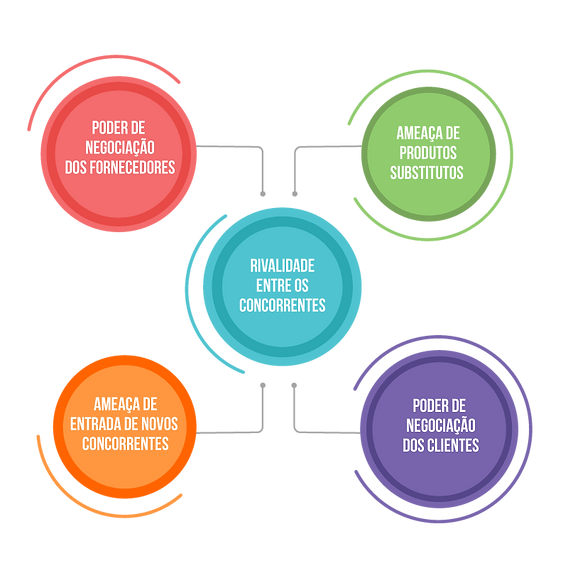
\includegraphics[width=0.8\linewidth]{7c8300_9e949360c69240ed92aab96ce376d792~mv2.png}
    \caption{Representação das forças de Porter\cite{imgporter}}
    \label{fig:forças-porter}
\end{center}


Um SI bem implementado cria barreiras de entrada para novos concorrentes. Por exemplo, empresas que operam com um TMS automatizado e integrado conseguem reduzir custos logísticos, oferecer melhores prazos e rastreabilidade, tornando difícil para novas empresas competirem nos mesmos níveis de eficiência e confiabilidade. O SI permite comparar preços e desempenhos de fornecedores com mais precisão, aumentando o poder da organização na negociação. Sistemas com dashboards analíticos fornecem indicadores de SLA (nível de serviço), custos por transporte e tempo médio de entrega, o que ajuda a selecionar e negociar com parceiros mais vantajosos. Ao oferecer serviços logísticos mais rápidos, transparentes e rastreáveis — habilitados por TMS e WMS —, a empresa aumenta o valor percebido pelo cliente. Isso reduz o poder de barganha dos clientes, pois ficam mais propensos a manter contratos com empresas que garantem confiabilidade e performance. A capacidade de inovação, habilitada por sistemas integrados com tecnologias como IoT e Machine Learning, diminui a atratividade de substitutos. Por exemplo, ao otimizar o tempo de entrega e reduzir erros operacionais, um SI torna mais difícil que um concorrente ofereça um serviço substituto com o mesmo custo-benefício. Os SIs aumentam a eficiência operacional e permitem diferenciação por meio da personalização de serviços logísticos, melhoria contínua baseada em dados e atendimento mais responsivo. Assim, mesmo em mercados saturados, as empresas que utilizam SIs conseguem se destacar pela performance, fidelizar clientes e operar com margens mais sustentáveis.

\section{Questões éticas}
\begin{center}
    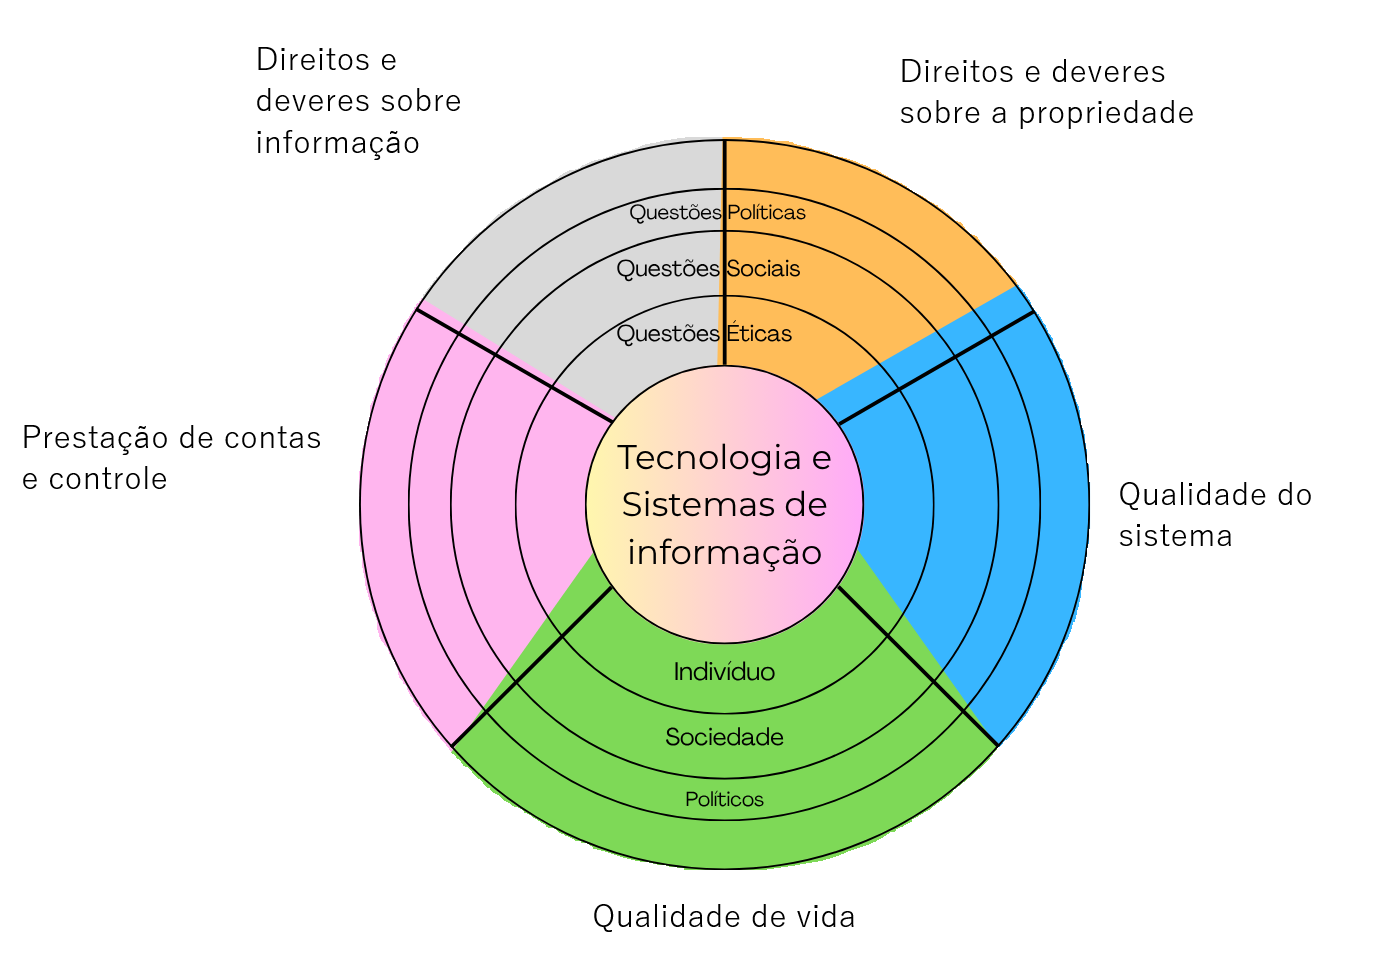
\includegraphics[width=0.8\linewidth]{Novos Concorrentes.png}
    \caption{Representação dos círculos concêntricos}
    \label{fig:circulos-concêntricos}
\end{center}
As questões éticas emergem de diversas em diversos contextos. Com base nos círculos concêntricos de Laudon \& Laudon é possível ver questões em diversos de seus níveis, o círculo atua como um lago inicialmente calmo, mas se perturbado este pode criar ondas e se espalhar partindo de questões individuais até a política.

Partindo do núcleo técnico, o sistema deve garantir segurança da informação e integridade dos dados, protegendo-os de possíveis vazamentos, ataques cibernéticos e modificações maliciosas ou acidentais que comprometam a confiança nos dados, elementos essenciais para a continuidade e credibilidade da operação logística.

Ao nível organizacional, há três elementos fundamentais a aplicação de boas práticas dentro do Sistema de informação; o treinamento de usuários, diz respeito à capacitação das pessoas que utilizarão o sistema, para que compreendam seu funcionamento, saibam operá-lo corretamente e extraiam o máximo de suas funcionalidades; a gestão da mudança, trata das estratégias adotadas para facilitar a transição de processos antigos para os novos, com o uso do sistema; e adoção consciente da automação, significa incorporar automações no sistema (como seleção automática de rotas ou geração de documentos fiscais) de forma planejada e ética, garantindo que os impactos sobre o trabalho humano sejam considerados.

No ambiente social, a preocupação com a privacidade dos dados de usuários é imprescindível para a operação do Sistema de Informação, dado que esses sistemas utilizam GPS e sensores para acompanhar em tempo real a localização de motoristas e operadores.

Chegando ao contexto político, existem diversas normas que regulam o transporte de mercadorias como emissão de notas fiscais eletrônicas (NF-e), documentos de transporte (CT-e, MDF-e), controle de jornada de motoristas, entre outras exigências. O sistema também deve se conformar a Lei Geral de Proteção de Dados (LGPD), lei que exige que qualquer sistema que armazene e processe dados pessoais adote medidas para garantir a privacidade, segurança e transparência no uso dessas informações.
\section{Conclusão}
O uso de Sistemas de Informação de Transporte de Mercadorias, como os TMS e WMS, é fundamental para enfrentar os desafios da logística moderna. Eles proporcionam vantagens competitivas por meio da eficiência, redução de custos e tomada de decisões mais embasadas, especialmente quando integrados a tecnologias avançadas como IoT, IA e Blockchain. Entender suas funcionalidades, arquitetura e impactos estratégicos é essencial para qualquer organização que deseja se destacar em um mercado altamente competitivo.
\nocite{*}
\bibliographystyle{IEEEtran}
\bibliography{referencias}
\end{document}
